\chapter{Future Work}
The prototype demonstrates end-to-end voting with identity unlinkability, double-vote prevention, and auditable tallies validated on a local blockchain. This chapter presents the validation results against the stated objectives, interprets the findings in terms of privacy and integrity guarantees, and identifies the steps required to evolve the system toward production readiness. The discussion is organised around three future directions: privacy hardening, deployment readiness, and hardware integration.
 
\section{Validation Results}
 
\subsection{Test Cases and Outcomes}
 
Table~\ref{tab:validation} summarises the test cases executed against the software prototype and their outcomes.
 
\begin{table}[htb]
\fontsize{10}{12}\selectfont
\caption{Validation test cases and outcomes}
\label{tab:validation}
\begin{tabular}{|p{5cm}|p{4cm}|p{3.5cm}|}
\hline
\textbf{Test Case} & \textbf{Expected Behaviour} & \textbf{Outcome} \\
\hline
Valid batch submission & Tallies incremented correctly & Pass \\\hline
Repeated identity hash in batch & Contract reverts transaction & Pass \\\hline
Invalid candidate \gls{id} in batch & Contract reverts transaction & Pass \\\hline
Vote submission below threshold & Buffer holds, no chain write & Pass \\\hline
Phase transition enforcement & Writes rejected outside Voting phase & Pass \\\hline
Results query post-submission & Correct aggregate counts returned & Pass \\
\hline
\end{tabular}
\end{table}
 
All six test scenarios produced the expected contract behaviour. Tally consistency was confirmed by comparing on-chain counts with the known contents of each submitted batch across multiple election runs.
 
\subsection{Anonymity Verification}
 
Post-submission inspection of on-chain state confirmed that no positional or temporal correspondence exists between the identity hash array and the candidate \gls{id} array. The on-chain record consists solely of a set of used hashes and a candidate-to-count mapping, with no per-vote entry, sequence number, or timestamp that could support re-identification. This satisfies the unlinkability requirement stated in Equation~\ref{eq:identity_hash} of Chapter~3.
 
\section{Interpretation of Results}
 
The results confirm that the two-stage batch submission model, combined with Fisher-Yates shuffling, effectively removes the on-chain basis for linkage attacks. The spent-key register provides deterministic double-vote prevention without storing any voter-identifiable data beyond the hash. The separation of concerns between the off-chain privacy layer and the on-chain integrity layer is validated as an effective design strategy for this threat model. The relayer remains the principal trust assumption: its correct and non-colluding behaviour is asserted rather than cryptographically proven in the current phase, which is the primary limitation of the prototype.
 
\section{Future Work}
 
\subsection{Privacy Hardening}
 
The most significant open item is eliminating the relayer as a single trust point. Introducing a zero-knowledge proof of shuffle correctness would allow any observer to verify that the candidate array was permuted honestly without the relayer revealing the permutation \cite{Wang2023}. Formal verification of the smart contract logic and an independent security audit are also planned to strengthen assurance of the double-vote and phase-guard mechanisms. Additional unlinkability mechanisms, such as commit-reveal schemes or threshold submission, will be evaluated under higher adversarial threat models.
 
\subsection{Deployment Readiness}
 
Hardening for real deployments requires strengthened key management for both the relayer signing key and the admin election-control key. Monitoring and structured logging should be added to support operational oversight without exposing sensitive data. Load testing under realistic voter arrival rates is needed to characterise buffer latency and determine appropriate threshold values. Auditability features for independent observers, such as Merkle-proof inclusion of batch hashes, are also planned.
\newpage
 
\subsection{Hardware Integration}
 
The planned hardware path moves identity capture and hashing from the browser to an \gls{rfid}-enabled ESP32-based polling terminal. Hardware-backed keys on the device would protect both voter credential capture and relayer signing, reducing the software attack surface. The terminal architecture is designed to preserve the same privacy guarantees validated in the software prototype: identity is hashed on-device and the raw credential never leaves the hardware boundary. Validating this equivalence through end-to-end testing on the hardware platform is the primary goal of the next project phase.
 
The prototype has demonstrated that a software-only, local-chain voting system can satisfy core requirements of voter anonymity, double-vote prevention, and auditable tallying. The validation results confirm the effectiveness of the batch shuffle and two-stage submission model against linkage attacks. Future work is prioritised around closing the relayer trust gap through cryptographic proofs, hardening the system for operational deployment, and integrating hardware-backed identity verification to extend the privacy boundary to the physical polling edge.
\begin{figure}[htbp]
    \centering
    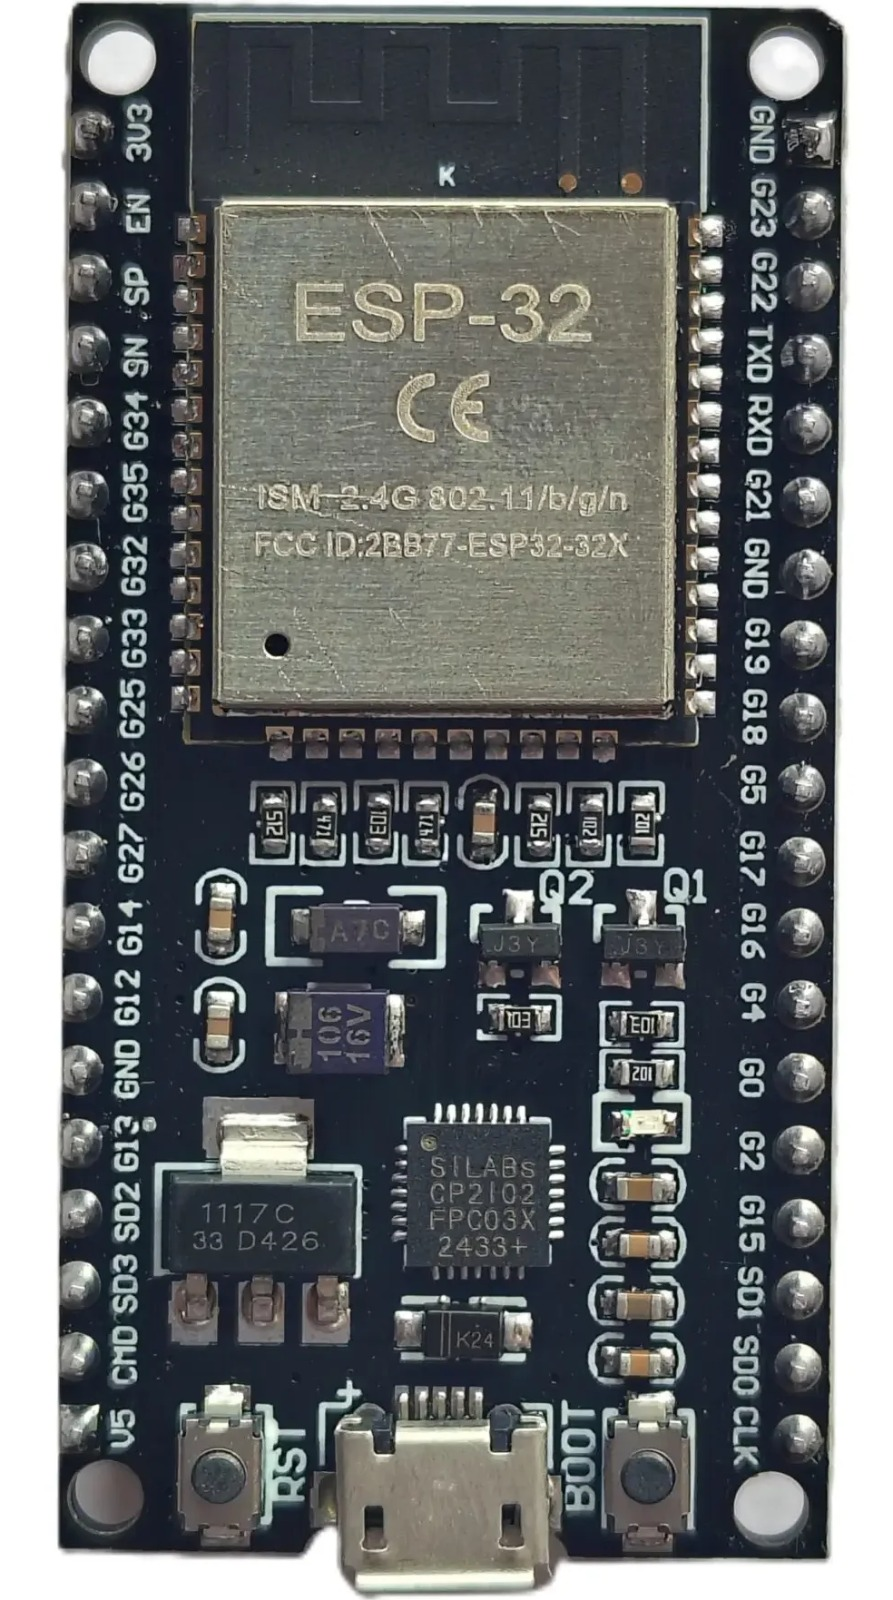
\includegraphics[width=0.2\linewidth]{Chapter5/5(1).jpeg}
    \caption{Microcontroller ESP32 (a)}
    \label{fig:Hardware Integration 1}
\end{figure}
\begin{figure}[htbp]
    \centering
    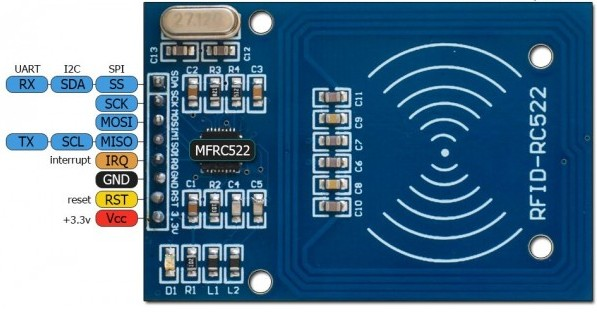
\includegraphics[width=0.4\linewidth]{Chapter5/5(2).jpeg}
    \caption{Microcontroller ESP32 (b)}
    \label{fig:Hardware Integration 2}
\end{figure}